\chapter{Método de Trabajo}
\label{chap:metodo}

\drop{E}{n} este capítulo se detalla la metodología utilizada para el desarrollo del presente \ac{TFG} así como las tecnologías utilizadas para llevar a término el proyecto.

Para la gestión y el desarrollo del \ac{TFG} se utilizará Kanban y \ac{TDD}, haciendo uso del desarrollo evolutivo.

Kanban proporciona un método productivo bien delineado en fases que garantiza que el cambio a la siguiente fase no se producirá hasta haberse completado correctamente la fase actual.

El desarrollo del producto software se realizará mediante \ac{TDD}, ya que es una solución que permite asegurarse del correcto funcionamiento de los componentes antes de permitir el siguiente paso.

Mediante el prototipado evolutivo conseguiremos ir perfilando el producto final mediante un acercamiento por fases terminadas.

Por tanto, el prototipado nos marcará la meta de cada fase, Kanban nos indicará los objetivos individuales necesarios para alcanzar el final de cada una de las fases y \ac{TDD} nos permitirá asegurarnos que los componentes desarrollados poseen la calidad exigida por Kanban para terminar el desarrollo del objetivo individual.


\section{Dispositivos empleados}
\label{dispositivos-empleados}
Para el desarrollo del \ac{TFG} se utilizarán los siguientes dispositivos:

	\subsection{Ordenador portátil}
	
	Para el desarrollo del TFG se ha utilizado un ordenador portátil con las características que se detallan en la tabla \ref{tab:portatil}.
	
	\begin{table}[H]
	  \centering 
	  \rowcolors{1}{gray!25}{white}
	  \begin{tabular}{p{0.4\linewidth}p{0.3\linewidth}}
	    \toprule
	    Fabricante 							& Acer 											\\
	    Modelo								& Aspire V 15 Nitro								\\
		Fabricante Procesador 				& Intel 										\\
		Modelo Procesador 					& i7-5500U 										\\
		Velocidad y Núcleos del Procesador & 2.4 GHz; 2 núcleos 							\\
		Memoria RAM 						& 16 \ac{GB} \ac{DDR}3L \ac{SDRAM} 			\\
		Disco Duro Principal y Secundario 	& 250 \ac{GB} \ac{SDD} y 1 \ac{TB} \ac{HDD}	\\
		Sistema Operativo					& Elementary \ac{OS} 							\\
	    \hline
	  \end{tabular}
	  \caption{Ordenador utilizado para el desarrollo \ac{TFG}}
	  \label{tab:portatil}
	\end{table}
	
	\subsection{Teléfono móvil}
	
	Para las pruebas del desarrollo en dispositivos móviles se ha utilizado un teléfono móvil con las características que se detallan en la tabla \ref{tab:movil}.
	
	\begin{table}[H]
	  \centering 
	  \rowcolors{1}{gray!25}{white}
	  \begin{tabular}{p{0.4\linewidth}p{0.3\linewidth}}
	    \toprule
	    Fabricante 				& LG 				\\
	    Modelo 					& D820 (Nexus 5) 	\\
		Fabricante Procesador 	& Qualcomm 			\\
		Modelo Procesador 		& Snapdragon 800 	\\
		Velocidad Procesador 	& 2.26 GHz 			\\
		Memoria RAM 			& 2 \ac{GB} 		\\
		Sistema Operativo 		& Android 6.0 		\\
		Tamaño Pantalla			& 4.95 pulgadas 	\\
	    \hline
	  \end{tabular}
	  \caption{Dispositivo móvil utilizado para el desarrollo \ac{TFG}}
	  \label{tab:movil}
	\end{table}

\section{Desarrollo evolutivo}
\label{section:desarrollo}
También conocido como prototipado evolutivo, este tipo de desarrollo se basa en exponer una implementación inicial al usuario permitiendo, a través de sus comentarios, refinar el sistema mediante versiones hasta alcanzar el producto final.
Este tipo de enfoque es más efectivo que un desarrollo en cascada debido a que satisface las necesidades inmediatas del cliente y debido a que utiliza un enfoque evolutivo, la especificación del producto se desarrolla de forma creciente en tanto en cuanto el cliente comienza a mejorar su comprensión y acercamiento al problema que pretende solucionar.
Debido a su propia naturaleza, el buen funcionamiento de este tipo de desarrollo, requiere de una gran vinculación por parte del cliente, que en este caso estará representado por el director del proyecto, ya que el elemento más importante en este prototipado, es la retroalimentación proveniente de numerosas entrevistas que ayuden a marcar el rumbo del desarrollo \cite{Somm06}.

\begin{figure}[H]
\centering
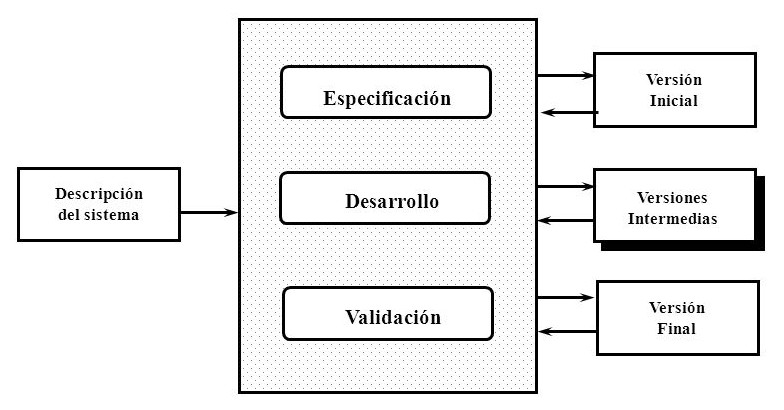
\includegraphics[width=120mm, fbox={\fboxrule} 4mm]{images/04-metodo/01-protipado_evolutivo.jpg}
\caption{Prototipado Evolutivo}
\label{fig:prototipado_evolutivo}
\end{figure}

\section{Kanban}
Kanban es una palabra japonesa que se deriva de \textit{kan} (visual) y \textit{ban} tarjeta. Se desarrolló como parte de una estrategia industrial japonesa para conseguir adecuar la producción a la demanda. Consiste en un sistema de visualización por medio de tarjetas de los recursos en procesos de producción.

Según Scrum Manager, una comunidad profesional para la difusión de Scrum, podríamos definir Kanban \cite{Pal15} de la siguiente manera:

\begin{tikzpicture}
	\node[shadowBox] {
	El término Kanban aplicado a la gestión ágil de proyectos se refiere a técnicas de representación visual de información para mejorar la eficiencia en la ejecución de las tareas de un proyecto.};
\end{tikzpicture}

Kanban se basa en un sistema de producción que dispara el trabajo solo cuando existe capacidad real para procesarlo \cite{Bahi11}. Este disparador está representado por las tarjetas Kanban, que están limitadas en número. Cada tarjeta representa un trabajo a realizar durante todo el proceso de desarrollo. Al llegar a la última fase, la tarjeta queda liberada para representar un nuevo trabajo.

Kanban mantiene únicamente tres reglas de funcionamiento, mostrar el proceso, limitar el trabajo en curso y optimizar el flujo de trabajo.

	\subsection{Mostrar el proceso}
	Consiste en la visualización de todo el proceso de desarrollo mediante un tablero físico (o un tablero virtual accesible por todas las partes, como es el caso de \href{https://trello.com/}{Trello}. El objetivo de este tablero es mejorar el entendimiento del proceso de trabajo actual, anticipar los posibles problemas y ayudar a la toma de decisiones resolutivas.
	Los tableros Kanban están formados por tres secciones, tal y como podemos ver en la figura \ref{fig:kanban_table_1}, \textit{To Do}, \textit{Doing} y \textit{Done}, que corresponden a la pila de entrada, el \ac{WIP} y la salida. Estas secciones se dividen en columnas representativas de los procesos de trabajo. En la figura \ref{fig:kanban_table_2} podemos ver un tablero típico con la pila de entrada (pending) y el \ac{WIP} (analysis, development, test y deploy).
	
	\begin{figure}[H]
	\centering
	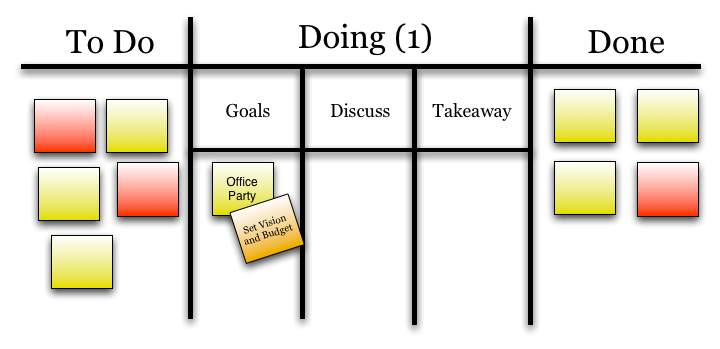
\includegraphics[width=120mm, fbox={\fboxrule} 4mm]{images/04-metodo/02-kanban_table_1.png}
	\caption{Secciones tablero Kanban}
	\label{fig:kanban_table_1}
	\end{figure}
	
	\begin{figure}[H]
	\centering
	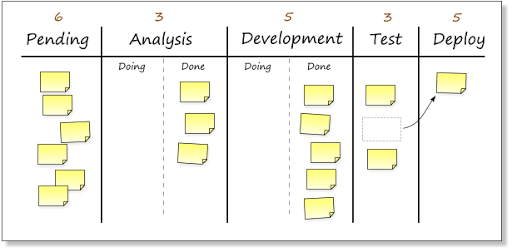
\includegraphics[width=120mm, fbox={\fboxrule} 4mm]{images/04-metodo/03-kanban_table_2.png}
	\caption{Columnas tablero Kanban}
	\label{fig:kanban_table_2}
	\end{figure}
	
	\subsection{Limitar el trabajo}
	Consiste en limitar la cantidad de ítems o tarjetas que pueden abordarse al mismo tiempo para un proceso definido, es decir, las columnas del tablero. Esta cantidad puede ser visualizada añadiendo el número máximo de tarjetas permitidas a cada columna como un número entre paréntesis al lado del nombre del proceso.
	Esta regla es muy útil para detectar rápidamente los posibles cuellos de botella que puedan producirse. En la imagen \ref{fig:kanban_table_3} podemos observar un desarrollo con un cuello de botella en el proceso \textit{Pruebas}.
	
	\begin{figure}[H]
	\centering
	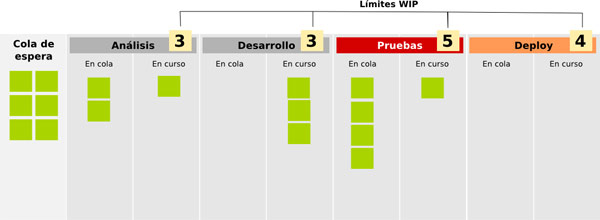
\includegraphics[width=120mm, fbox={\fboxrule} 4mm]{images/04-metodo/04-kanban_table_3.jpg}
	\caption{Cuello de botella en Kanban}
	\label{fig:kanban_table_3}
	\end{figure}

\section{\acs{TDD}}
	\acf{TDD} es una metodología de desarrollo ágil consistente en escribir primero las pruebas para después implementar el código necesario para pasarlas satisfactoriamente. Según Carlos Blé \cite{Ble10}, podríamos definirlo como:
	
	\begin{tikzpicture}
	\node[shadowBox] {
	\ac{TDD} es una técnica para diseñar software que se centra en tres pilares fundamentales:
	\begin{itemize}[label={$\bullet$},labelindent=\parindent,leftmargin=2cm]
		\item La implementación de las funciones justas que el cliente necesita.
		\item La minimización del número de defectos que llegan a la fase de producción.
		\item La producción de software modular, altamente reutilizable y preparado para el cambio.
	\end{itemize}
	};
\end{tikzpicture}

	\subsection{Algoritmo \ac{TDD}}
	El algoritmo para realizar \ac{TDD} consta únicamente de tres pasos (ver figura \ref{fig:tdd_algorithm}):
	
	\begin{enumerate}
		\item Escribir el test para el requisito a desarrollar elegido
		\item Implementar el código necesario para pasar el test
		\item Refactorizar el código para eliminar duplicidades y mejorarlo.
	\end{enumerate}
	
	\begin{figure}[H]
	\centering
	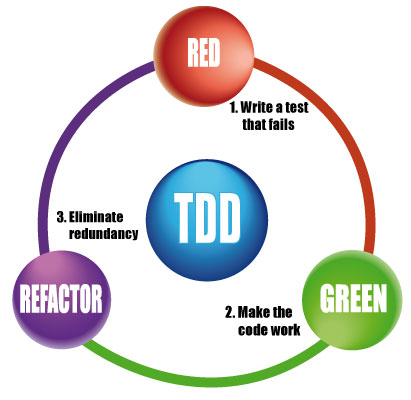
\includegraphics[height=80mm, fbox={\fboxrule} 4mm]{images/04-metodo/05-tdd.jpg}
	\caption{Algoritmo TDD}
	\label{fig:tdd_algorithm}
	\end{figure}
	
	\subsection{Ventajas de usar \ac{TDD}}
	Según Kent Beck \cite{Beck04}, creador de TDD, estas son algunas de las principales ventajas de su uso:
	
	\begin{itemize}[label={$\bullet$},labelindent=\parindent,leftmargin=2cm]
		\item La calidad del software aumenta.
		\item Escribir el test antes que el código obliga a escribir el mínimo de funcionalidad necesaria evitando diseños innecesarios.
		\item Los test son la mejor documentación técnica para consultar qué misión cumple cada parte del código.
	\end{itemize}
	

\section{Marco tecnológico}
En esta sección se incluyen las herramientas y tecnologías utilizadas para el desarrollo del \ac{TFG}.

	\subsection{Sistema Operativo}
		\subsubsection{Elementary OS}
			El sistema operativo utilizado para el desarrollo del proyecto es \textit{\href{https://elementary.io/}{Elementary OS}}. Elementary	es un sistema operativo basado en Ubuntu, a su vez basado en Debian que usa como entorno de escritorio \ac{GNOME}. Al estar basada en Ubuntu es completamente compatible con los repositorios y paquetes de este sistema hasta el punto de usar el \textit{Centro de Software de Ubuntu}.
			Uno de los puntos más fuertes de esta distribución es su gran estabilidad y la interfaz amigable y visualmente atractiva que presenta. Actualmente, este sistema operativo ha sido descargado cinco millones de veces \cite{Garc15}, lo que supone una quinta parte de las descargas totales de la distribución madre (Ubuntu) y existen unos 400.000 usuarios activos \cite{Agud15}.	
	
	\begin{figure}[H]
	\centering
	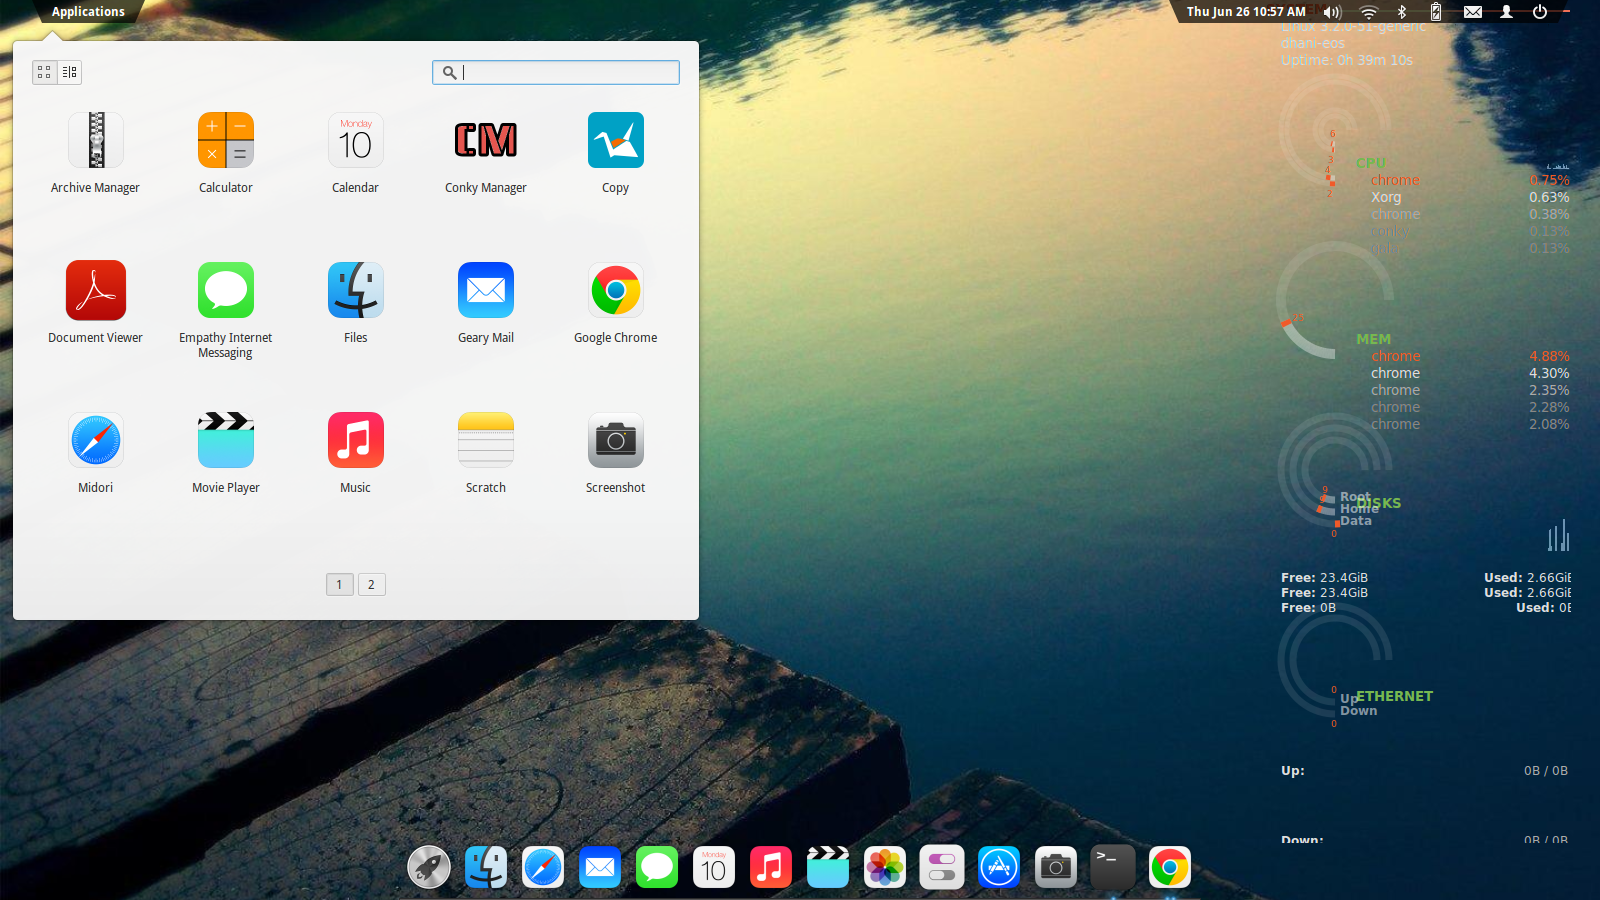
\includegraphics[width=120mm, fbox={\fboxrule} 4mm]{images/04-metodo/11-elementary_preview.png}
	\caption{Previsualización de Elementary OS}
	\label{fig:elementary-preview}
	\end{figure}
	
	\begin{figure}[H]
	\centering
	
\includegraphics[width=40mm, fbox={\fboxrule} 4mm]{images/04-metodo/12-elementary_logo.jpg}
	\caption{Logo Elementary OS}
	\label{fig:elementary-logo}
	\end{figure}
	
			\subsubsection{Microsoft Windows 10}
			Este sistema operativo se utilizará de manera auxiliar debido a que algunas de las herramientas software utilizadas únicamente están disponibles para sistemas operativos Windows.
			La versión 10 del sistema operativo de Microsoft devuelve el protagonismo a los teclados y ratones, perdido en la versión 8 y recuperado parcialmente en la versión 8.1. También destacable es la vuelta del menú inicio a través del conocido botón en la esquina inferior derecha.
			
			\begin{figure}[H]
			\centering
			
\includegraphics[width=40mm, fbox={\fboxrule} 4mm]{images/04-metodo/13-windows_logo.png}
			\caption{Logo Microsoft Windows 10}
			\label{fig:windows-logo}
			\end{figure}
			

	\subsection{Herramientas de diseño}
		\subsubsection{Visual Paradigm}
		Visual Paradigm es una herramienta \ac{UML} \ac{Case} para el modelado de sistemas con soporte para \ac{UML} 2.
		Esta herramienta se utilizará para el modelado de los diagramas \ac{UML} necesarios para la consecución del \ac{TFG}.
		Las principales características de esta aplicación son la creación de modelos \ac{UML} con compatibilidad con la versión 2.1 del lenguaje de modelado, el modelado de bases de datos, la interoperabilidad con intercambio de modelos con otras herramientas, el modelado de requerimientos y la generación automática de código y documentación.
		
		\begin{figure}[H]
		\centering
		
\includegraphics[width=40mm, fbox={\fboxrule} 4mm]{images/04-metodo/14-visual_paradigm_logo.jpg}
		\caption{Logo Visual Paradigm}
		\label{fig:visual-paradigm-logo}
		\end{figure}
		
		\subsubsection{Gantt Project}
		Es una herramienta utilizada para la creación de diagramas de Gantt, lo que permitirá planificar y organizar el trabajo necesario para la consecución del \ac{TFG}.
		Sus principales características son la posibilidad de importar y exportar archivos de Microsoft Project, la creación de diagramas PERT y la exportación a archivos \ac{PNG}, \ac{PDF} y \ac{HTML},
		
		\begin{figure}[H]
		\centering
		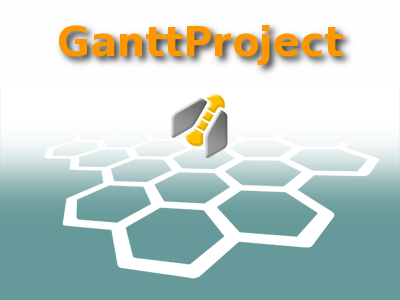
\includegraphics[width=40mm, fbox={\fboxrule} 4mm]{images/04-metodo/15-gantt_project_logo.png}
		\caption{Logo Gantt Project}
		\label{fig:gantt-project-logo}
		\end{figure}
		
		\subsubsection{Moqups}		
		\href{https://moqups.com}{Moqups} es una herramienta online utilizada para la realización de bocetos, maquetación y prototipados rápidos. Su gran ventaja es la cantidad de herramientas que dispone así como el número de plantillas y formas predeterminadas.
			
		\begin{figure}[H]
		\centering
		
\includegraphics[width=40mm, fbox={\fboxrule} 4mm]{images/04-metodo/16-moqups_logo.png}
		\caption{Logo Moqups}
		\label{fig:gantt-project-logo}
		\end{figure}
		
		\begin{figure}[H]
		\centering
		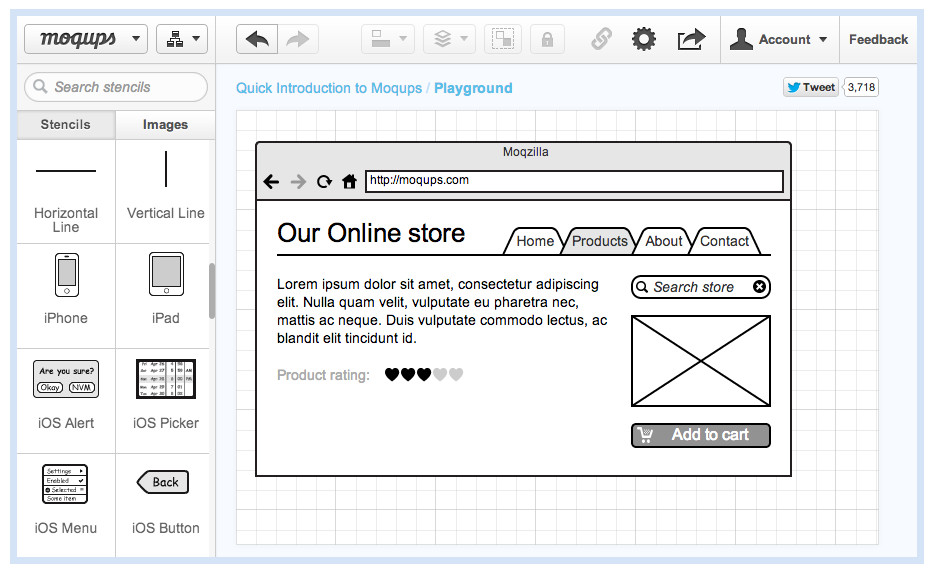
\includegraphics[width=120mm, fbox={\fboxrule} 4mm]{images/04-metodo/17-moqups_preview.jpg}
		\caption{Previsualización Moqups}
		\label{fig:gantt-project-logo}
		\end{figure}
		
	\subsection{Herramientas de gestión del proyecto}
		\subsubsection{Git}
		Git es un software de control de versiones diseñado por el también creador de Linux, Linus Torvalds. El control de versiones consiste en la gestión y administración de los cambios realizados sobre los archivos involucrados en el desarrollo del presente \ac{TFG}. Permite conocer el estado del proyecto, los cambios que se han realizado, quién los realizó y en qué momento y hacer una regresión completa a cualquier estado anterior entre otras características.
		Git es uno de los gestores de control de versiones más conocidos y utilizados, junto con \textit{\ac{SVN}} y \textit{Mercurial}.
		
		\begin{figure}[H]
		\centering
		
\includegraphics[width=40mm, fbox={\fboxrule} 4mm]{images/04-metodo/18-git_logo.png}
		\caption{Logo Git}
		\label{fig:git-logo}
		\end{figure}
		
		\subsubsection{Github}
		\label{subsubsection:github}
		Github es un servicio de alojamiento gratuito de repositorios git. En la versión gratuita todos los proyectos son públicos y se hace necesario el contrato de un plan de pago para poder configurar un acceso privado.
		Git y Github son utilizados en el presente \ac{TFG} para establecer un control de versiones en línea, de manera que la comunicación en cuanto a código operativo entre el director y el autor del \ac{TFG}, sea lo más fluida posible.
		
		\begin{figure}[H]
		\centering
		
\includegraphics[width=40mm, fbox={\fboxrule} 4mm]{images/04-metodo/19-github_logo.jpg}
		\caption{Logo Github}
		\label{fig:github-logo}
		\end{figure}
	
		\subsubsection{Trello}
		\label{subsubsection:trello}
		Trello es una herramienta colaborativa utilizada para organizar proyectos mediante tableros. Es ampliamente utilizada en el ámbito empresarial para organizar el trabajo a realizar. Debido a sus particularidades, Trello se sincroniza perfectamente con el método Kanban. En el presente \ac{TFG} se utilizará para la ordenación de trabajo y el seguimiento necesario por parte del director hacia el autor.
		
		\begin{figure}[H]
		\centering
		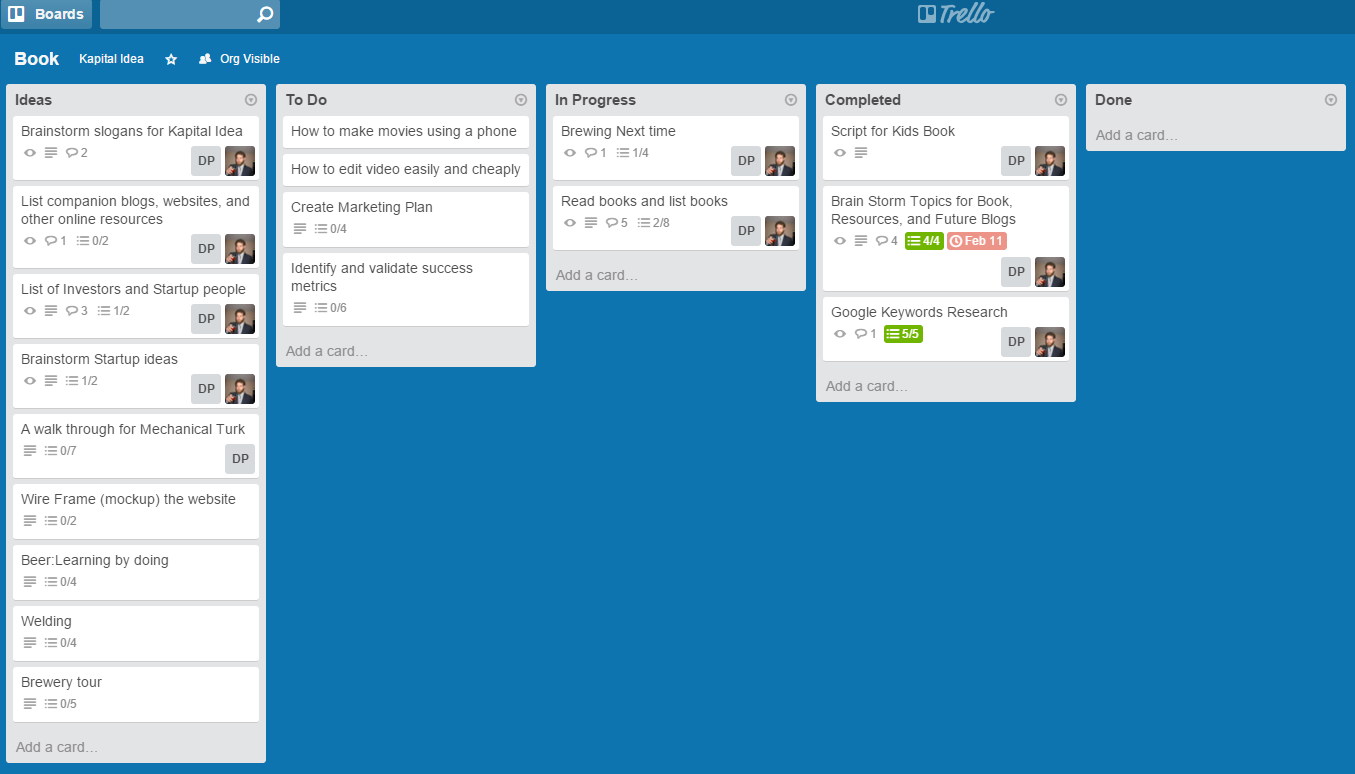
\includegraphics[width=120mm, fbox={\fboxrule} 4mm]{images/04-metodo/20-trello_preview.png}
		\caption{Previsualización de Trello}
		\label{fig:trello-preview}
		\end{figure}
		
		\begin{figure}[H]
		\centering
		
\includegraphics[width=40mm, fbox={\fboxrule} 4mm]{images/04-metodo/21-trello_logo.jpg}
		\caption{Logo Trello}
		\label{fig:trello-logo}
		\end{figure}
		
	\subsection{Herramientas, tecnologías y frameworks para el desarrollo}
		\subsubsection{Ruby}
		Ruby es un lenguaje de programación orientado a objetos creado por Yukihiro Matsumoto, también conocido como Matz. La principal característica que posee es que absolutamente todo es un objeto, incluso lo que en otros lenguajes se definen como \textit{tipos primitivos}. Al crear el lenguaje, Matz se inspiró en Python y Perl intentando que el protagonismo sea la diversión y la productividad del desarrollador \cite{Yuki20}, enfatizando el hecho de que el diseño de sistemas debe prestar más atención a las necesidades humanas que a las necesidades de las máquinas.
		
		\begin{figure}[H]
		\centering
		
\includegraphics[width=40mm, fbox={\fboxrule} 4mm]{images/04-metodo/06-ruby_logo.png}
		\caption{Logo Ruby}
		\label{fig:ruby-logo}
		\end{figure}
		
		\subsubsection{Rails}
		Rails es un framework de desarrollo web escrito en Ruby siguiendo el paradigma \ac{MVC} (ver figura \ref{fig:mvc}). Se basa en dos principios fundamentales, \textit{\ac{DRY}} (no te repitas), esto es, escribir el mismo código una y otra vez es una mala praxis y \textit{Convención sobre Configuración} que permite que Rails suponga que quieres hacer y como quieres hacerlo en función de las prácticas habituales de programación. Se utilizará para el desarrollo de la herramienta web.
		
		\begin{figure}[h!btp]
		\centering
		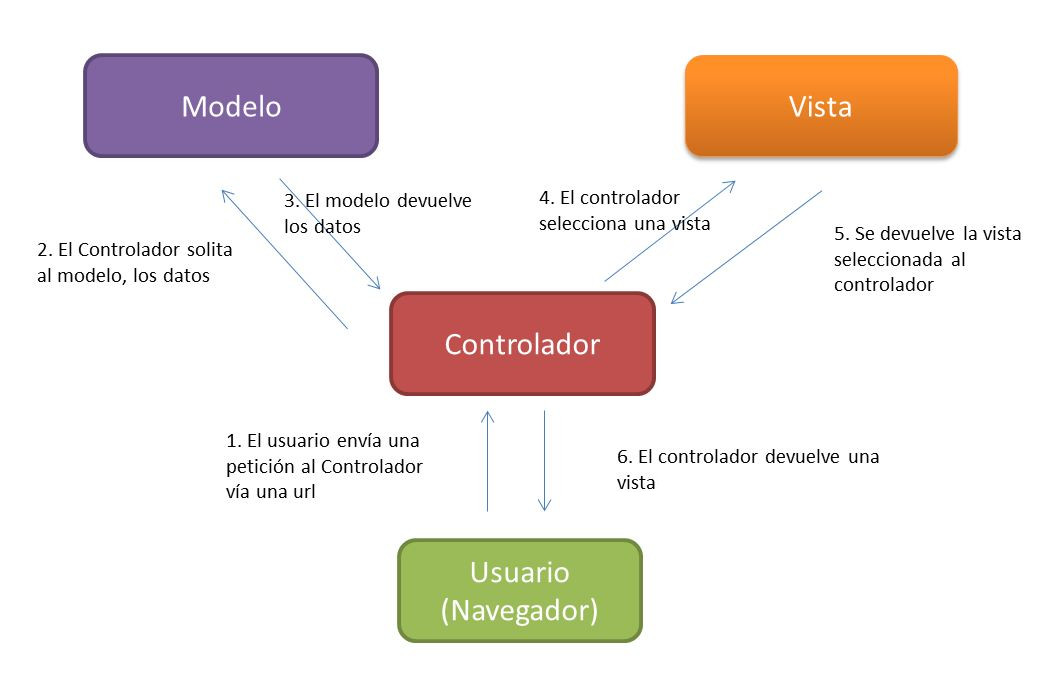
\includegraphics[width=120mm, fbox={\fboxrule} 4mm]{images/04-metodo/07-mvc.jpg}
		\caption{Modelo Vista Controlador}
		\label{fig:mvc}
		\end{figure}
		
		\begin{figure}[H]
		\centering
		
\includegraphics[width=40mm, fbox={\fboxrule} 4mm]{images/04-metodo/08-rails_logo.png}
		\caption{Logo Rails}
		\label{fig:rails-logo}
		\end{figure}
		
		\subsubsection{Android}
		Android es un sistema operativo desarrollado inicialmente para móviles que utiliza los kernel de Linux como núcleo del mismo. Durante el año 2014 alcanzo una cuota de mercado del 63 \% (ver figura \ref{fig:os-mobile}. Fuente \cite{Are15})por lo que puede considerarse el más importante de los sistemas operativos móviles. 
		La aplicación móvil se desarrollará para este sistema operativo, utilizando para ello el lenguaje Java.
		
		\begin{figure}[h!btp]
		\centering
		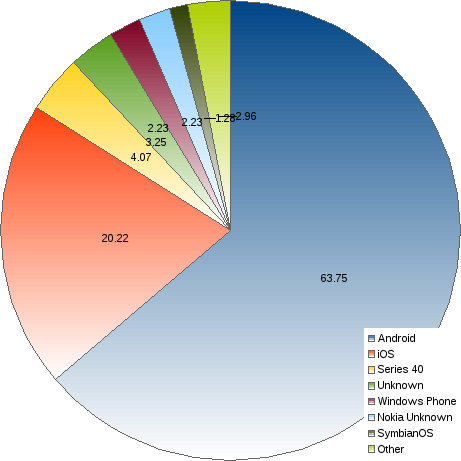
\includegraphics[width=60mm, fbox={\fboxrule} 4mm]{images/04-metodo/09-os_mobile.png}
		\caption{Cuota de mercado de los sistemas operativos móviles}
		\label{fig:os-mobile}
		\end{figure}
		
		\begin{figure}[H]
		\centering
		
\includegraphics[width=40mm, fbox={\fboxrule} 4mm]{images/04-metodo/10-android_java.jpg}
		\caption{Logo Android y Java}
		\label{fig:android-java-logo}
		\end{figure}
		
		\subsubsection{AngularJS}
		AngularJS es un framework de JavaScript utilizado en el lado del cliente de la aplicación. Ha sido desarrollado por Google y es una \textit{ampliación} de la sintaxis existente en \ac{HTML} para mejorar su funcionalidad, ya que los creadores no creen que este lenguaje esté aún preparado para servir vistas dinámicas eficientemente. Utiliza el patrón \ac{MVC}.
		
		\begin{figure}[H]
		\centering
		
\includegraphics[width=40mm, fbox={\fboxrule} 4mm]{images/04-metodo/22-angularjs_logo.png}
		\caption{Logo AngularJS}
		\label{fig:angularjs-logo}
		\end{figure}

		\subsubsection{Bootstrap}
		Bootstrap es un framework \ac{CSS} desarrollado en el año 2011 por Twitter. El código fue liberado y actualmente está accesible en Github. Permite la creación de interfaces limpias y funcionales y mantiene un diseño \textit{responsive} o adaptativo, esto es, adopta automáticamente el tamaño adecuado al dispositivo en el que debe mostrarse.
		
		\begin{figure}[H]
		\centering
		
\includegraphics[width=40mm, fbox={\fboxrule} 4mm]{images/04-metodo/23-bootstrap_logo.png}
		\caption{Logo Bootstrap}
		\label{fig:bootstrap-logo}
		\end{figure}
		
		\begin{figure}[H]
		\centering
		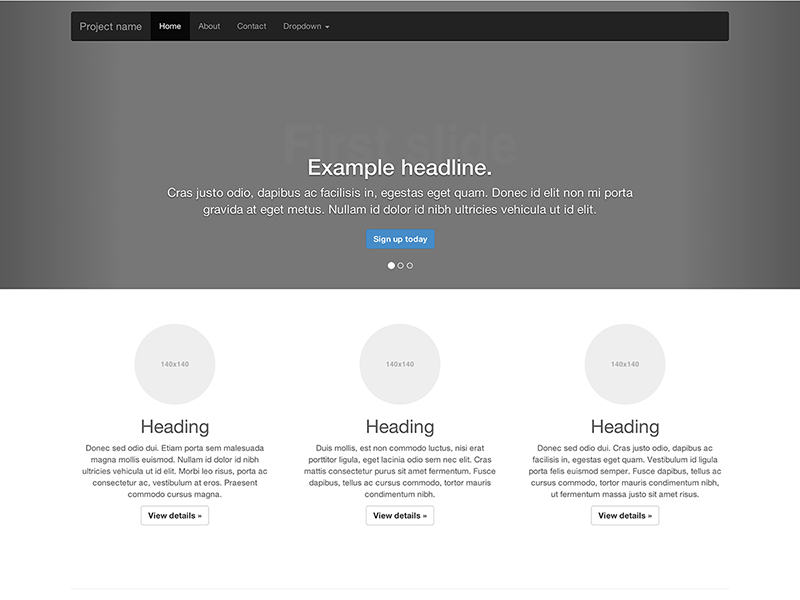
\includegraphics[width=120mm, fbox={\fboxrule} 4mm]{images/04-metodo/24-bootstrap_preview.jpg}
		\caption{Previsualización de Bootstrap}
		\label{fig:bootstrap-preview}
		\end{figure}
		
		\subsubsection{Rspec}
		Rspec es una libreria para Ruby diseñada para la realización de pruebas. Actualmente es una de las herramientas más populares para este cometido en Ruby. Su diseño está enfocado tanto a la productividad como a la comodidad y diversión del desarrollador.

		\begin{figure}[H]
		\centering
		
\includegraphics[width=40mm, fbox={\fboxrule} 4mm]{images/04-metodo/25-rspec_logo.png}
		\caption{Logo Rspec}
		\label{fig:rspec-logo}
		\end{figure}
		
		\subsubsection{\ac{HTML}}
		\ac{HTML} es un lenguaje de marcado utilizado para la creación y diseño de páginas web. Es un estándar a cargo de \ac{W3C}. La interpretación del código corre a cargo del navegador web. En octubre de 2014 se publico la versión definitiva de la nueva revisión, \ac{HTML}5.
		
		\begin{figure}[H]
		\centering
		
\includegraphics[width=40mm, fbox={\fboxrule} 4mm]{images/04-metodo/26-html_logo.png}
		\caption{Logo HTML5}
		\label{fig:html5-logo}
		\end{figure}
		
		\subsubsection{\ac{CSS}}
		Es un mecanismo para describir cómo va a mostrarse un documento, ofreciendo a los desarrolladores el control sobre el formato de los documentos. Se utiliza para concretar el estilo de los documentos \ac{HTML}. Actualmente está en su tercera versión, \ac{CSS}3.

		\begin{figure}[H]
		\centering
		
\includegraphics[width=40mm, fbox={\fboxrule} 4mm]{images/04-metodo/27-css3_logo.png}
		\caption{Logo CSS3}
		\label{fig:css3-logo}
		\end{figure}	
		
		\subsubsection{\ac{JSON}}
		\ac{JSON} es un formato para el intercambio de datos nacido como alternativa a \ac{XML}. Una de sus mayores ventajas es que puede leerse con cualquier lenguaje de programación, por lo que es usado para el intercambio de información entre distintos sistemas. El funcionamiento básico para formar estructuras de datos válidas, es mediante pares clave-valor.
		
		\begin{figure}[H]
		\centering
		
\includegraphics[width=40mm, fbox={\fboxrule} 4mm]{images/04-metodo/28-json_logo.png}
		\caption{Logo JSON}
		\label{fig:json-logo}
		\end{figure}	
		
		\subsubsection{Sublime Text 3}
		\textit{Sublime Text 3} es un editor de texto y código fuente escrito en \textit{C++}. Originalmente era una extensión de \textit{Vim}, que a su vez es una versión mejorada de \textit{Vi}, un editor de texto presente en los sistemas UNIX.
		Este programa será el utilizado para la escritura del código necesario durante la elaboración del \ac{TFG}.
		
		\begin{figure}[H]
		\centering
		
\includegraphics[width=40mm, fbox={\fboxrule} 4mm]{images/04-metodo/29-sublime_text_logo.png}
		\caption{Logo Sublime Text 3}
		\label{fig:sublime-text-logo}
		\end{figure}
		
		\subsubsection{Midori}
		Es el navegador web ligero por defecto de Elementary OS con un motor principal basado en Webkit, conocido por la estabilidad de los navegadores Safati, Chrome y Opera. Se utilizará para el acceso a la aplicación web. Debido a que usa \ac{GTK} como interfaz gráfica puede ejecutarse sin errores en escritorios basados en  como \ac{GNOME} o Xfce.
		Ofrece compatibilidad con HTML5 y CSS3.
		
		\begin{figure}[H]
		\centering
		
\includegraphics[width=40mm, fbox={\fboxrule} 4mm]{images/04-metodo/30-midori_logo.png}
		\caption{Logo Midori}
		\label{fig:midori-logo}
		\end{figure}
		
		\subsubsection{Chromium}
		Es un navegador web de código abierto basado en Google Chrome.
		Tiene un diseño minimalista y su motor principal está basado en Webkit. La mayor parte de este proyecto está bajo licencia BSD, lo que permite el uso parcial o total de su código fuente. Su punto fuerte consiste en su estabilidad, debido a que usa un proceso para cada pestaña, el bloqueo de uno de ellos no afecta al funcionamiento general del programa.
		Ofrece compatibilidad con HTML5 y CSS3.
		
		\begin{figure}[H]
		\centering
		
\includegraphics[width=40mm, fbox={\fboxrule} 4mm]{images/04-metodo/39-chromium_logo.png}
		\caption{Logo Chromium}
		\label{fig:chromium-logo}
		\end{figure}
		
		\subsubsection{Mozilla Firefox}		
		Es uno de los navegadores más conocidos y usados, junto con Internet Explorer y Google Chrome, está desarrollado mediante una licencia de código abierto.
		Es compatible con los principales lenguajes de programación web y destaca su velocidad y estabilidad.

		\begin{figure}[H]
		\centering
		
\includegraphics[width=40mm, fbox={\fboxrule} 4mm]{images/04-metodo/38-firefox_logo}
		\caption{Logo Mozilla Firefox}
		\label{fig:firefox-logo}
		\end{figure}
		
	\subsection{Herramientas para la gestión de bases de datos}
		\subsubsection{MongoDB}
		Es una base de datos NoSQL, orientada a documentos, esto es, en vez de guardar los datos en registros los guarda en documentos en una representación binaria de \ac{JSON} conocida como \ac{BSON}. La principal diferencia con las bases de datos relacionales, es que no resulta necesario seguir un mismo esquema para una misma colección (concepto similar a las tablas de las bases de datos relacionales).
		
		\begin{figure}[H]
		\centering
		
\includegraphics[width=40mm, fbox={\fboxrule} 4mm]{images/04-metodo/31-mongodb_logo.png}
		\caption{Logo MongoDB}
		\label{fig:mongodb-logo}
		\end{figure}	
		
		\subsubsection{MongoLab}
		MongoLab nos permite el uso de una base de datos como servicio \ac{SaaS}, usando para ello la infraestructura proporcionada por distintos proveedores como Google, Amazon o Microsoft.
				
		\begin{figure}[H]
		\centering
		
\includegraphics[width=40mm, fbox={\fboxrule} 4mm]{images/04-metodo/33-mongolab-logo.png}
		\caption{Logo MongoLab}
		\label{fig:mongolab-logo}
		\end{figure}
		
		\subsubsection{RoboMongo}
		RoboMongo es un administrador gráfico de bases de datos MongoDB que permite mantener múltiples conexiones a las bases de datos, bien a través del servidor local, bien a través de MongoLab.
		
		\begin{figure}[H]
		\centering
		
\includegraphics[width=40mm, fbox={\fboxrule} 4mm]{images/04-metodo/32-robomongo_logo.png}
		\caption{Logo Robomongo}
		\label{fig:robomongo-logo}
		\end{figure}
	
	\subsection{Herramientas documentales}
		\subsubsection{TexMaker}
		TexMaker es un editor gráfico para lenguaje LaTex distribuido bajo licencia \textit{\ac{GPL}}. Existen versiones disponibles para Microsoft Windows, Linux / Unix y Mas OsX. Permite la edición de texto automático mediante asistentes configurables y la detección y manejo de los errores es rápida y sencilla.
				
		\begin{figure}[H]
		\centering
		
\includegraphics[width=40mm, fbox={\fboxrule} 4mm]{images/04-metodo/34-texmaker_logo.png}
		\caption{Logo Texmaker}
		\label{fig:texmaker-logo}
		\end{figure}
		
		\subsubsection{\ac{GIMP}}
		\ac{GIMP} es un editor de imágenes tanto en mapa de bits como en dibujos y fotografías, libre y gratuito. Forma parte del proyecto \ac{GNU} y se publica bajo la misma licencia. Es uno de los programas de manipulación e gráficos más utilizado y probablemente el más usado en entornos GNU / Linux. Se utilizará para la modificación, edición y creación de imágenes para el presente \ac{TFG}.
		
		\begin{figure}[H]
		\centering
		
\includegraphics[width=40mm, fbox={\fboxrule} 4mm]{images/04-metodo/35-gimp_logo.png}
		\caption{Logo \ac{GIMP}}
		\label{fig:gimp-logo}
		\end{figure}
		
		\subsubsection{Microsoft Visio}
		Es un software de dibujo vectorial para el sistema operativo Windows que permite la realización de diversos tipos de diagramas. 
		
		\begin{figure}[H]
		\centering
		
\includegraphics[width=40mm, fbox={\fboxrule} 4mm]{images/04-metodo/36-visio_logo.jpg}
		\caption{Logo Microsoft Visio}
		\label{fig:visio-logo}
		\end{figure}
	
	\subsection{Herramientas de implantación}
		\subsubsection{Heroku}
		\label{subsubsection:heroku}
		Heroku es un servicio \ac{PaaS} utilizado para el despliegue de aplicaciones en línea desarrolladas, entre otros lenguajes, en Ruby.
				
		\begin{figure}[H]
		\centering
		
\includegraphics[width=40mm, fbox={\fboxrule} 4mm]{images/04-metodo/37-heroku_logo.png}
		\caption{Logo Heroku}
		\label{fig:heroku-logo}
		\end{figure}
	

% Local Variables:
%  coding: utf-8
%  mode: latex
%  mode: flyspell
%  ispell-local-dictionary: "castellano8"
% End:
